\chapter{Anforderungsanalyse}
\label{cha:Anforderungsanalyse}

In diesem Kapitel werden funktionale und nichtfunktionale Anforderungen an das zu entwickelnde System ermittelt. Zu diesem Zweck werden Anwendungsfälle definiert und in Beziehung zueinander gesetzt. Außerdem werden die Möglichkeiten ausgewählter Technologien für die Realisierung der Server- und Clientkomponente betrachtet und bewertet.

\section{Funktionale Anforderungen}
\label{sec:Funktionale Anforderungen}

Ziel ist die Entwicklung einer Webanwendung, die die folgenden Spezifikationen und Schnittstellen unter Berücksichtigung der Rahmenbedingungen (siehe Abschnitt \ref{sec:Analyse:Nichtfuntionale Anforderungen}) implementiert. Die ermittelten funktionalen Anforderungen und deren Abhängigkeiten zueinander sind Gegenstand der Abbildung \ref{fig:usecase}. 

\begin{figure}[H]
\centering
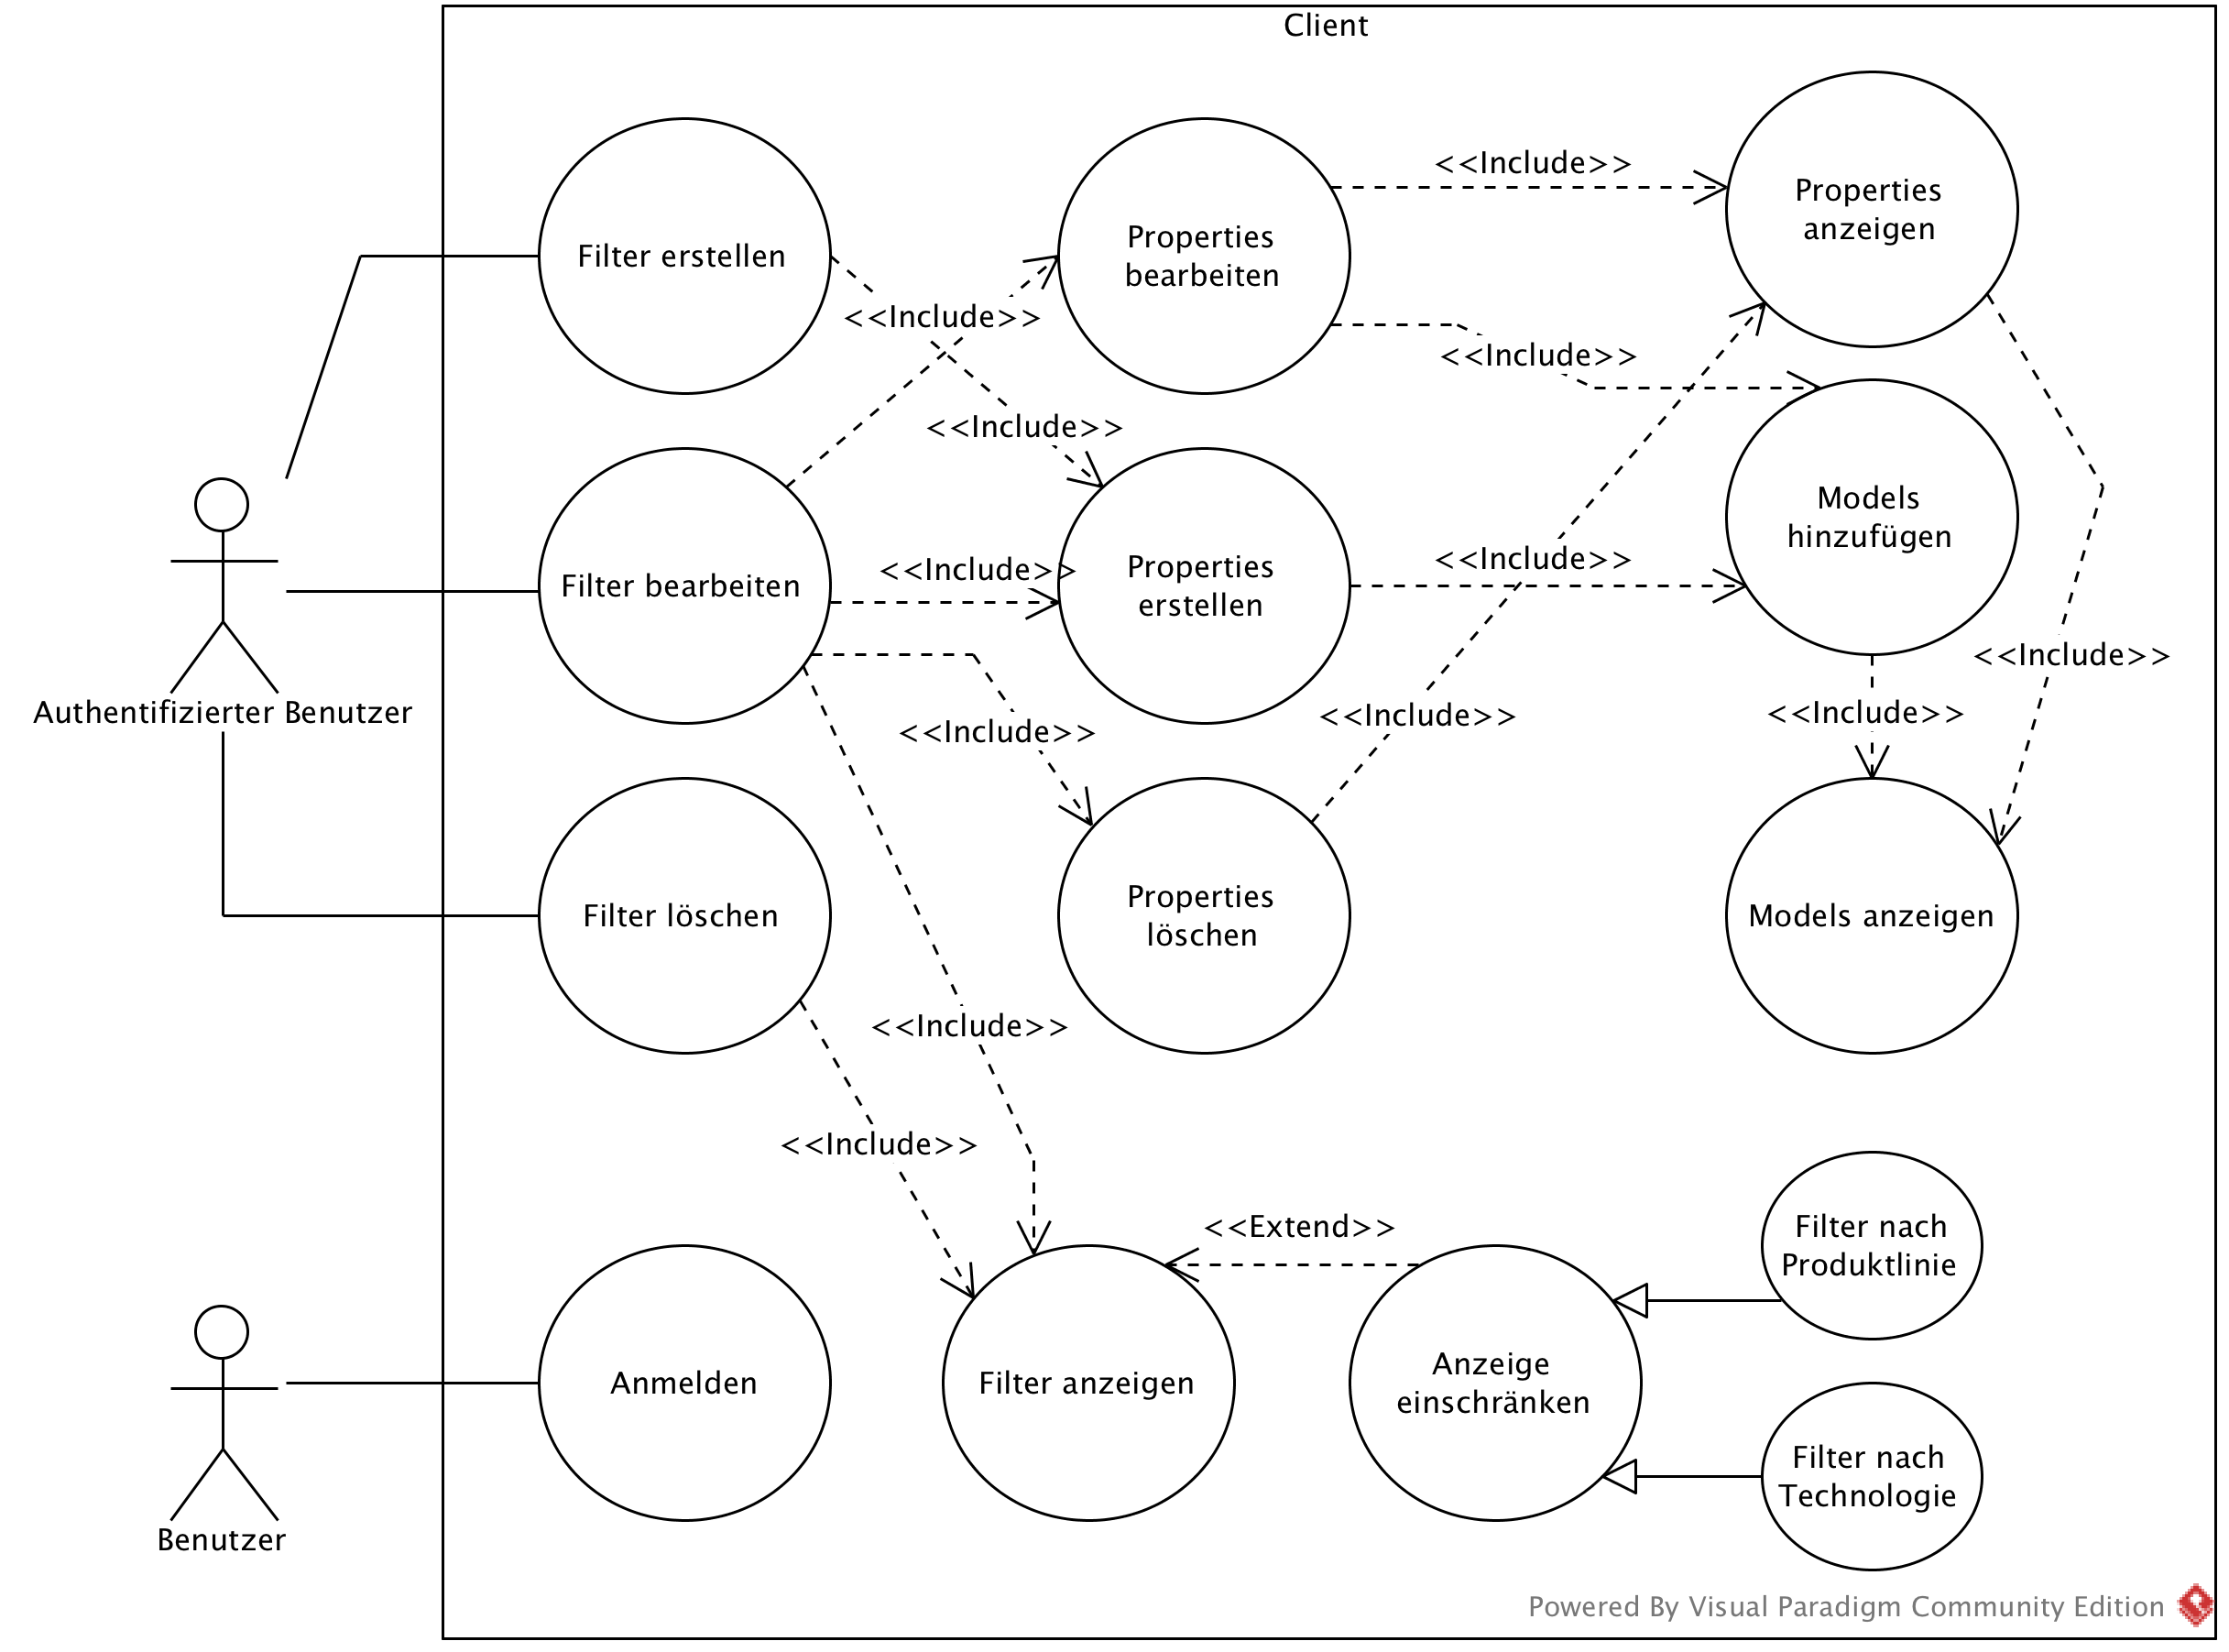
\includegraphics[width=.95\textwidth]{usecase} %{CS0031}
\caption{Anwendungsfalldiagramm}
\label{fig:usecase}
\end{figure}

Für das Verständnis der ermittelten Anwendungsfälle ist es notwendig, Filter als zentrale Objekte der Webanwendung zu verstehen. In Abschnitt \ref{sec:Zielsetzung} wurden Filter bereits als Elemente der Benutzeroberfläche eingeführt, denen eine komplexe Datenstruktur zugrunde liegt. Diese Datenstruktur beinhaltet sowohl Verknüpfungen zu Produkten und Produkteigenschaften, als auch layoutspezifische Daten, die das Erscheinungsbild in der Benutzeroberfläche bestimmen. Aufgrund dieser vielschichtigen Verknüpfungen können die Filter nur in Teilabschnitten bearbeitet werden. Dieser Sachverhalt wurde bei der Erarbeitung der Anwendungsfälle berücksichtigt und Abhängigkeiten modelliert.

\subsubsection{/F1.1/ Anmelden}

\begin{description}[leftmargin=8em,style=nextline]
\item[Akteure] Benutzer
\item[Includes] Keine
\item[Beschreibung]
Um die Anwendung zu nutzen, muss sich der Benutzer mit Benutzernamen und Passwort anmelden. Die Anmeldedaten müssen über eine Anmeldemaske eingegeben und anschließend verifiziert werden. Nach erfolgreicher Anmeldung muss der Benutzer in den geschützten Bereich der Webanwendung weitergeleitet werden.
\end{description}

\subsubsection{/F2.1/ Filter anzeigen}

\begin{description}[leftmargin=8em,style=nextline]
\item[Akteure] Authentifizierter Benutzer
\item[Includes] Keine
\item[Beschreibung]
Filtersteuerelemente müssen dem Benutzer angezeigt werden. Die Anwendung generiert die Filtersteuerelemente anhand der Filterdaten und orientiert sich dabei am Layout des FlowConfigurator. Die Anzeige muss zusätzlich Schaltflächen für die auf die Filter anwendbaren Operationen enthalten (Bearbeiten, Löschen, Erstellen).
\end{description}

\subsubsection{/F2.2/ Filteranzeige einschränken}

\begin{description}[leftmargin=8em,style=nextline]
\item[Akteure] Authentifizierter Benutzer
\item[Extends] F2.1 
\item[Beschreibung]
Der Benutzer muss die Möglichkeit haben, die angezeigten Filter einzuschränken. Die Filterung soll nach Technologie und Produktlinie möglich sein. Die Anwendung zeigt dazu entsprechende Steuerelemente an.
\end{description}

\subsubsection{/F2.3/ Filter erstellen}

\begin{description}[leftmargin=8em,style=nextline]
\item[Akteure] Authentifizierter Benutzer
\item[Includes] F3.3
\item[Beschreibung]
Der Benutzer kann neue Filter hinzufügen. Die Anwendung stellt dem Benutzer zu diesem Zweck Dateneingabemasken zur Verfügung. Das Hinzufügen der Filter erfolgt in Teilabschnitten, durch die der Benutzer geführt wird:

\begin{itemize}
\item Die Filtergruppe muss festgelegt werden (Basis- oder Spezialfilter)
\item Der Filtertyp muss bestimmt werden (Boolean oder Listenfilter) 
\item Geräteeigenschaften und Sensoren, nach denen gefiltert werden soll, müssen bestimmt bzw. verknüpft werden
\end{itemize}

\end{description}

\subsubsection{/F2.4/ Filter bearbeiten}

\begin{description}[leftmargin=8em,style=nextline]
\item[Akteure] Authentifizierter Benutzer
\item[Includes] F2.1, F3.2, F3.3, F3.4
\item[Beschreibung]
Der Benutzer muss existierende und neu angelegte Filter vollumfänglich bearbeiten können. Dazu werden von der Anwendung Dateneingabemasken angeboten. Zusätzlich soll auch die Anordnung der Filtersteuerelemente in der Benutzeroberfläche anpassbar sein. 
\end{description}

\subsubsection{/F2.5/ Filter löschen}

\begin{description}[leftmargin=8em,style=nextline]
\item[Akteure] Authentifizierter Benutzer
\item[Includes] F2.1
\item[Beschreibung]
Der Benutzer muss Filter über die Benutzeroberfläche löschen können. Dazu werden entsprechende Schaltflächen in der Filterübersicht angezeigt.
\end{description}

\subsubsection{/F3.1/ Properties anzeigen}

\begin{description}[leftmargin=8em,style=nextline]
\item[Akteure] Authentifizierter Benutzer
\item[Includes] F4.1
\item[Beschreibung]
Properties müssen in der Benutzeroberfläche angezeigt werden. Der Benutzer muss die Möglichkeit haben über Schaltflächen Aktionen auf den Properties auszuführen (Bearbeiten, Löschen, Erstellen).
\end{description}

\subsubsection{/F3.2/ Properties bearbeiten}

\begin{description}[leftmargin=8em,style=nextline]
\item[Akteure] Authentifizierter Benutzer
\item[Includes] F4.1, F4.2
\item[Beschreibung]
Properties beziehen sich auf Sensorspezifikationen, nach denen gefiltert werden soll. Der Benutzer muss vorhandene Properties eines Filters über eine Dateneingabemaske bearbeiten können.
\end{description}

\subsubsection{/F3.3/ Properties erstellen}

\begin{description}[leftmargin=8em,style=nextline]
\item[Akteure] Authentifizierter Benutzer
\item[Includes] F4.2
\item[Beschreibung]
Der Benutzer muss ebenso neue Properties zu einem Filter hinzufügen können. Die Anwendung stellt zu diesem Zweck eine Dateneingabemaske zur Verfügung.
\end{description}

\subsubsection{/F3.4/ Properties löschen}

\begin{description}[leftmargin=8em,style=nextline]
\item[Akteure] Authentifizierter Benutzer
\item[Includes] F3.1
\item[Beschreibung]
Der Benutzer muss Properties über die Benutzeroberfläche löschen können. Dazu werden entsprechende Schaltflächen in der Property-Übersicht angezeigt.
\end{description}

\subsubsection{/F4.1/ Models anzeigen}

\begin{description}[leftmargin=8em,style=nextline]
\item[Akteure] Authentifizierter Benutzer
\item[Includes] Keine
\item[Beschreibung]
Alle verfügbaren Models müssen aufgelistet werden. Aufgrund der Vielzahl der Models müssen diese für den Benutzer organisiert werden. Zu diesem Zweck stellt die Anwendung eine mehrseitige und sortierbare Tabelle bereit. 
\end{description}

\subsubsection{/F4.2/ Models hinzufügen}

\begin{description}[leftmargin=8em,style=nextline]
\item[Akteure] Authentifizierter Benutzer
\item[Includes] F4.1
\item[Beschreibung]
Models sind Sensoren, die mit einer Property verknüpft werden. Der Benutzer muss bestehende Models mit einer Property verknüpfen können. Die Anwendung stellt dafür eine Übersicht zur Verfügung, die es den Benutzer erlaubt über eine Checkbox Models an- und abzuwählen.
\end{description}

\section{Nichtfunktionale Anforderungen}
\label{sec:Analyse:Nichtfuntionale Anforderungen}

Neben der Umsetzung der funktionalen Anforderungen, sollen für die Umsetzung der zu entwickelnden Webanwendung folgende Qualitätsanforderungen beachtet werden:

\subsubsection{Performance}

Aufgrund des Umfangs der zu bearbeitenden Daten und die zu erwartenden Latenzen ist es notwendig, die Schnittstelle möglichst leichtgewichtig zu konzipieren. Weiterhin ist es notwendig, Geschäftsprozesse weitestgehend serverseitig zu realisieren. Serverseitige Ressourcen sollen bei Bedarf skaliert werden können, um die Performance zu verbessern.

\subsubsection{Benutzbarkeit und Layout}
\label{sec:Analyse:Benutzbarkeit und Layout}

Gemessen am Funktionsumfang sollte die zu entwickelnde Webanwendung ein möglichst simples, strukturiertes und bedienerfreundliches Layout besitzen. Das Layout soll sich dabei allgemein an dem der FlowConfigurator Software orientieren, um für den Benutzer ein gewohntes Umfeld zu schaffen. Eine Besonderheit ergibt sich durch das anzuwendende \ac{WYSIWYG}-Prinzip: Die Anzeige und Darstellung der Filtersteuerelemente in der Filterübersicht müssen hinsichtlich der Anordnung und Gruppierung möglichst exakt der Benutzeroberfläche des FlowConfigurator entsprechen. Nach dem Rückführen der Filterdaten in den FlowConfigurator müssen die Filtersteuerelemente dort genau so ausgeprägt und angeordnet sein, wie sie der Benutzer zuvor in der Webanwendung vorgefunden hat.

Die neu zu gestaltenden Dateneingabemasken sollen für die jeweiligen Anwendungsfälle (siehe Abschnitt \ref{sec:Funktionale Anforderungen}) auf eigenen Unterseiten bereitgestellt werden, die über eine Navigation miteinander verknüpft sind. Dabei gilt es eine gewisse Konsistenz hinsichtlich des Aussehens und der Bedienung zu gewährleisten. 

\subsubsection{Sicherheit}

Da es sich bei den zu verarbeitenden Daten um nicht öffentliche Geschäftsdaten handelt, muss die Webanwendung Mechanismen zur Absicherung implementieren. Der Benutzer muss sich mit Benutzernamen und Passwort an der Webanwendung anmelden, um diese zu nutzen. Zusätzlich muss der Zugriff auf die Schnittstelle, welche die Daten zur Verfügung stellt, serverseitig abgesichert werden um Missbrauch vorzubeugen.

\subsubsection{Portabilität}

Die Webanwendung soll so konzipiert werden, dass die einzelnen Komponenten austauschbar sind. Das bedeutet, dass in jedem Fall eine lose Kopplung zwischen Komponenten gegeben sein soll. Die Schnittstellenspezifikation sollte aus diesem Grund allgemein gehalten werden, um eine Wiederverwendbarkeit in möglichen Folgeprojekten zu gewährleisten.

Zusätzlich soll die Benutzeroberfläche auf verschiedenen Bildschirmgrößen korrekt dargestellt werden. Der Schwerpunkt liegt aber in der Unterstützung gebräuchlicher Desktop-Bildschirmgrößen.

\section{Technologiebewertung und -entscheidung}
\label{sec:Analyse:Technologiebewertung und -entscheidung}

\subsection{Server}
\label{sec:Analyse:Server}

Für die Realisierung der Anwendung müssen einige technologische Grundvoraussetzungen erfüllt werden. Die ermittelten Kriterien werden in Tabelle \ref{tab:Technologiebewertung} mit den ausgewählten Plattformen NodeJS, PHP und C\# (CSharp) abgeglichen. Die Auswahl der Plattformen, die zum Vergleich herangezogen werden, erfolgt anhand von Kenntnissen und Erfahrungen, die der Autor dieser Arbeit bereits mit den Plattformen gemacht hat. Objektiv betrachtet gibt es natürlich auch noch weitere infrage kommende Plattformen, wie zum Beispiel Java oder Ruby on Rails. Aufgrund des begrenzten Zeitrahmens dieser Arbeit ist es aber notwendig, Vorkenntnisse des Autors zu berücksichtigen, um eine möglichst zeiteffiziente Entwicklung zu gewährleisten. Der Vergleich konkreter Frameworks entfällt, da es ausschließlich um die Bewertung technischer Grundvoraussetzungen geht.

\begin{table}[H]
\centering
\def\rr{\rightskip=0pt plus1em \spaceskip=.3333em \xspaceskip=.5em\relax}
\setlength{\tabcolsep}{1ex}
\def\arraystretch{1.20}
\setlength{\tabcolsep}{1ex}
\small
\begin{tabular}{|r||c|c|c|} \hline
& \emph{NodeJS} & \emph{PHP} & \emph{C\#} \\
\hline\hline
MSSQL-Unterstützung & \checkmark & \checkmark & \checkmark \\
\hline
Plattformunabhängigkeit & \checkmark & \checkmark & $\times$ \\
\hline
Database First & \checkmark & \checkmark & \checkmark \\
\hline
\end{tabular}
\caption{Technologiebewertung auf Grundlage technischer Grundanforderungen}
\label{tab:Technologiebewertung}
\end{table}

\subsubsection{MSSQL-Unterstützung}

Die bereitgestellte Datenbank basiert auf \acf{MSSQL}. Deshalb ist es notwendig, dass die ausgewählte Technologie, Treiber zum Ansprechen dieser Datenbank bereitstellt. Diese Anforderung wird Unteranderem auch gestellt, weil eine MSSQL-Datenbank im Umfeld einer Webanwendung einen geringeren Verbreitungsgrad hat und eine Treiber-Unterstützung daher nicht selbstverständlich ist. Alle zum Vergleich stehenden Technologien erfüllen formal diese Anforderung. Die Treiberunterstützung unter C\# ist dabei aufgrund der Nähe zum Microsoft-Ökosystem sehr robust und unterstützt auch die aktuellsten SQL-Server Versionen. Der MSSQL-Treiber für NodeJS und PHP bauen beide auf dem \ac{TDS} Protokoll auf, das ursprünglich von Sybase entwickelt und später von Microsoft übernommen wurde. Es gibt verschiedene Ausbaustufen des Protokolls und auch Open-Source Ableger, wie zum Beispiel FreeTDS. Die \ac{MSSQL}-Treiber für PHP und NodeJS werden aber direkt von Microsoft bereitgestellt.

\subsubsection{Plattformunabhängigkeit}

Die Entwicklung unter C\# impliziert die Bindung an das Microsoft-Ökosystem. Entwicklungsumgebung, Technologiestack und Serverbetriebssystem werden dabei vorgegeben. Daraus ergeben sich die Nachteile, dass die Entwicklung der Anwendung nur unter dem Windows Betriebssystem stattfinden kann und eine Windows-Serverumgebung für die Bereitstellung der Anwendung benötigt wird. Auf NodeJS und PHP basierende Plattformen können unter allen gängigen Betriebssystemen entwickelt werden. Die Bereitstellung kann dabei auf vergleichsweise günstigen Linux-Servern erfolgen.

\subsubsection{Database First}

\ac{ORM} ist eine Technik der Softwareentwicklung, mit der eine, in einer objektorientierten Programmiersprache programmierte, Anwendung, Objekte in einer relationalen Datenbank ablegen kann. Die Anwendung sieht die Datenbank dann als objektorientierte Datenbank, was die Programmierung erleichtert. \parencite[vgl.][511]{Vogel2011} Die Implementierung eines \ac{ORM}-Frameworks ist generell für alle Anwendungen mit objektorientiertem Hintergrund empfehlenswert. Im Kontext dieser Arbeit ergibt sich aber eine Besonderheit. Es existiert bereits eine umfangreiche Datenbasis, aus denen ORM-Modelklassen abgeleitet werden müssen. Aufgrund des vergleichsweise großen Umfangs ist es aufwendig, diese Klassen händisch anzulegen. Eine Modelklasse modelliert neben Attributen, Relationsschemata und Relationsnamen auch die Beziehungen zu anderen Tabellen, die je nach Datenbasis sehr komplex ausfallen können. Diese Beziehungen aus einer bestehenden Datenbasis händisch in die entsprechenden Modelklassen zu übertragen würde viel Zeit in Anspruch nehmen und aufgrund der Komplexität zu Fehlern führen. Deshalb ist es notwendig, die Modelklassen aus der Datenbank vollautomatisch zu generieren. Dieses Prinzip wird auch als Database First bezeichnet und von den meisten ORM-Frameworks bereits nativ unterstützt. In Fällen, wo keine native Unterstützung vorgesehen ist, gibt es zahlreiche Erweiterungen für bekannte ORM-Frameworks, die sich dieser Problematik widmen.

NodeJS bietet mit der Bibliothek sequelize-Auto eine Erweiterung für das ORM-Framework sequelize an. Das umfangreiche Entity-Framework auf Basis von C\# bietet von Haus aus eine Funktion zur Generierung von Models aus einer Datenbank. Das in der PHP-Welt weitverbreitete Doctrine ORM-Framework bietet ebenfalls native Unterstützung zur Generierung der Modelklassen an. Weiterhin gibt es auch Erweiterungen für das PHP-basierte Eloquent ORM-Framework.

\subsection{Client}
\label{sec:Analyse:Client}

Der Webclient wird ausschließlich über eine einheitliche Schnittstelle mit dem Server kommunizieren. Daher haben die Technologieanforderungen, die für die Serverkomponenten ermittelt wurden, keine Auswirkung auf die Technologieentscheidung des Webclients. Als Kommunikationsprotokoll kommt für Webanwendungen standardmäßig \ac{HTTP} zum Einsatz. Die Benutzeroberfläche wird mittels HTML, CSS und Javascript realisiert. Damit ergeben sich keine besonderen Anforderungen bezüglich des eingesetzten Frameworks. Populäre Javascript Frameworks wie zum Beispiel AngularJS, Ember oder Backbone eignen sich alle gleichermaßen gut, um sowohl die Schnittstelle anzusprechen, als auch die ermittelten funktionalen und nichtfunktionalen Anforderungen umzusetzen. Javascript wird heutzutage aber nicht mehr nur eingesetzt um Benutzerinteraktionen auszuwerten, Inhalte zu verändern, nachzuladen oder zu generieren und so die Möglichkeiten von HTML und CSS zu erweitern, sondern findet auch außerhalb von Browsern als Servertechnologie Anwendung. Daraus ergeben sich Synergien mit der in Abschnitt \ref{sec:Analyse:Server} betrachteten serverseitigen NodeJS Plattform, die ebenfalls auf Javascript basiert. Der Einsatz ein und derselben Sprache für die Entwicklung von Client und Server kann die Realisierung aufgrund des geteilten Technologie-Stacks\footnote{Ein Technologie-Stack bezeichnet alle in einem Projekt benutzten Technologien} beschleunigen, da die Komplexität verringert und Abhängigkeiten reduziert werden.

\subsection{Machbarkeitsstudie}

Die in Abschnitt \ref{sec:Analyse:Server} gewonnenen Erkenntnisse aus dem Vergleich von ausgewählten Serverplattformen basieren lediglich auf Recherchen und sind damit nicht verifiziert. Vor allem wenn für die Sicherstellung technischer Grundvoraussetzungen im Rahmen der Projektanforderungen Open-Source Bibliotheken eingesetzt werde müssen, kann auf die versprochenen Funktionalitäten nicht uneingeschränkt vertraut werden. Das kann sowohl an unvollständigen Dokumentationen liegen, die keine gesicherten Rückschlüsse auf die benötigte Funktionalität zulassen, als auch an Unzuverlässigkeiten und Fehlern in den Implementierungen.

Um die Erkenntnisse aus der Technologierecherche zu verifizieren ist es notwendig die getätigten Annahmen anhand von prototypischen Implementierungen zu überprüfen. Als Schwerpunkt wird dabei die MSSQL Treiberunterstützung und die Generierung der ORM-Modelklassen nach dem Database First Prinzip getestet. Dabei gibt es keinen speziellen Projektrahmen; es werden stets nur die nötigsten Voraussetzungen geschaffen um eine gesicherte Annahme über die Funktionsfähigkeit der zu testenden Implementierungen tätigen zu können. Dabei kommen sogenannte \emph{Seeds} zum Einsatz. Als Seeds im Kontext der Software-Entwicklung werden vorkonfigurierte Projekte bezeichnet, die für nahezu alle populären Plattformen und Frameworks zur Verfügung stehen. Diese Projekte implementieren bereits benötigte Abhängigkeiten, die für die Realisierung vieler Projekte ohnehin gebraucht werden. Meist sind das Implementierungen für den Zugriff auf Datenbanken, darauf aufbauende rudimentäre Benutzerauthentifizierung, sowie einfache HTML-Templates. Dieses Vorgehen beschleunigt die Machbarkeitsstudie, da keine komplizierten Projektkonfigurationen vorgenommen werden müssen.

\subsubsection{NodeJS}

Für den Test der MSSQL-Anbindung wurde das Beispielprojekt \emph{express-example}\footnote{Siehe \hyperlink{https://github.com/sequelize/express-example}{https://github.com/sequelize/express-example}} verwendet. Express, ist der dabei der Name eines serverseitigem Frameworks auf Basis von NodeJS. Dieses Projekt beinhaltet das ebenfalls auf NodeJS basierende ORM-Framework \emph{sequelize}. Das Projekt ist für die Benutzung einer MySQL-Datenbank vorkonfiguriert. Die benötigten Treiber für die MSSQL-Unterstützung müssen nachinstalliert werden. Es wird dabei der offiziell von Microsoft bereitgestellten Treiber für NodeJS verwendet.

Nach der erfolgreichen Installation muss die im Projekt enthaltende Konfigurationsdatei mit den Verbindungsdaten der bereitgestellten Testdatenbank erweitert werden. Der Datenbankdialekt wird außerdem von MySQL auf MSSQL geändert. Die Testdatenbank ist eine Spiegelung der von der netbase Gmbh zur Verfügung gestellten Datenbank. Für den Test der Datenbankanbindungen werden jeweils nur sehr einfache Abfragen zum Lesen, Schreiben und Löschen von Datensätzen implementiert. Die Tests ergeben eine fehlerfreie Funktion der verwendeten MSSQL-Treiber.

Als nächstes wird zum Test des Database First Prinzips das Projekt um das Paket \emph{sequelize-auto} erweitert. Laut Dokumentation soll es damit möglich sein, ORM-Modelklassen auf Grundlage der Testdatenbank zu generieren. Angesteuert wird die Bibliothek innerhalb der Projektumgebung über die Kommandozeile, indem die korrekten Verbindungsdaten übergeben werden. Als Ergebnis des Tests werden zwar alle ORM-Modelklassen mit den korrekten Schemata generiert, aber es fehlt die Modellierung der Beziehung der Tabellen. Dieser Sachverhalt ist aus der Dokumentation nicht ersichtlich und konnte anhand weiterer Recherchen als fehlendes Feature identifiziert werden. Es können außerdem keine alternativen Bibliotheken zur Bereitstellung der benötigten Funktionalität gefunden werden.

\subsubsection{PHP}

Als Ausgangsbasis für die PHP-Tests dient das Framework Laravel. Die MSSQL-Treiberunterstützung wird auf Basis des im Laravel Framework enthaltenen ORM-Frameworks \emph{Eloquent} getestet. Verwendet wird der offizielle von Microsoft bereitgestellte MSSQL-Treiber. Die Basis der Testumgebung bildet PHP in der Version 5.6.24. Es werden ebenfalls einfache Abfragen zum Lesen, Schreiben und Löschen von Datensätzen implementiert. Dabei kann eine einwandfreie Treiberunterstützung verifiziert werden.

Für die Generierung der Modelklassen wird das Projekt um die Bibliothek \emph{laravel-model-generator} erweitert. Diese Bibliothek wird ebenfalls über die Kommandozeile angesprochen und bietet umfangreiche Einstellungsmöglichkeiten, die eine feingranulare Konfiguration der zu generierenden ORM-Modelklassen zulässt. Die Modelklassen können generiert werden und modellieren nach einer stichprobenartigen Kontrolle die korrekten Schemata und Beziehungen der Testdatenbank. Ein Problem konnte bei der Modellierung von zusammengesetzten Primärschlüsseln identifiziert werden. Diese fehlen bei der Generierung und müssen händisch nachgetragen werden.

\subsection{Ergebnis}

Anhand der in Abschnitt \ref{sec:Analyse:Technologiebewertung und -entscheidung} getätigten theoretischen Bewertungen technologischer Grundvoraussetzungen und der im Anschluss durchgeführten Machbarkeitsstudie konnte eine Entscheidung hinsichtlich der einzusetzenden Technologie getroffen werden. Die Entwicklung des Prototyps mit C\# kann aufgrund der vom Autor aufgestellten Anforderung der Plattformunabhängigkeit nicht erfolgen. Die Plattform NodeJS bietet interessante Synergien zwischen einem auf Javascript basierenden Client-Frontend und einer ebenfalls auf Javascript basierenden Serverplattform. Die getätigte Annahme über die Unterstützung des Database First Prinzips konnte allerdings mittels der durchgeführten Machbarkeitsstudie widerlegt werden. Die für die Serverplattform PHP getätigten Annahmen und die erfolgreich verlaufende Machbarkeitsstudie führt zu der Entscheidung PHP als Serverplattform einzusetzen. Aufgrund der Erfahrungen des Autors und der vielversprechend verlaufenden Machbarkeitsstudie wird das PHP Framework Laravel die Basis der Serverkomponente bilden.

Für die Realisierung des Frontend kommt AngularJS als Javascript-Framework zum Einsatz. Die Entscheidung beruht auf den bereits gemachten positiven Erfahrungen des Autors mit AngularJS und den unkritischen technologischen Anforderungen. Es ist anzumerken, dass auf Grundlage der gestellten Anforderungen, auch die in Abschnitt \ref{sec:Analyse:Client} genannten Alternativen hätten eingesetzt werden können.